\documentclass[myposter,portrait]{sciposter}

%% uzitocne package
\usepackage{multicol}
\usepackage{color}
\usepackage{graphicx}

%% znaky s diakritikou
%\usepackage[utf8]{inputenc}
%\usepackage[T1]{fontenc}
% \usepackage[slovak]{babel} % slovenske delenie slov

%% definicia farieb
\definecolor{mainCol}{rgb}{0.91,0.82,0.74} % farba pozadia posteru
\definecolor{sectionCol}{rgb}{0,0,0} % farba nadpisu
\definecolor{textCol}{rgb}{0.2,0,0} % farba hlavneho textu
\definecolor{BoxCol}{rgb}{1,1,0.8} % farba boxu okolo nadpisov

\def\mysection#1{
{\color{sectionCol}\section*{\sc\bfseries #1}}}

\usepackage{fontspec}
\usepackage{polyglossia}
\setdefaultlanguage{english}
\usepackage{csquotes}
\usepackage{microtype}

\usepackage{minted}
\usemintedstyle{tango}

\usepackage{fancyvrb}
\usepackage{qrcode}
\usepackage{tikz}

\begin{document}
\setlength{\logowidth}{20cm}
\setlength{\titlewidth}{\textwidth}
\addtolength{\titlewidth}{-\logowidth}
\rightlogo[0.9]{fmfilogo-farebne}
\useleftlogofalse

%\color{textCol}

\title{Evaluation of SAT-based\\ preimage attack optimizations}
\author{Ladislav P\'apay\\
        Supervisor: Martin Stanek}
\institute{%
Katedra informatiky, 
FMFI UK, Mlynská Dolina, 842~48~Bratislava
}
\maketitle

%%TODOLIST
% remove python/oo details
% replace something with a diagram?

\begin{multicols*}{3}
%\mysection{Introduction}
SAT solvers are a universal tool for finding solutions to boolean satisfiability problems.
In the past they have been used for cryptographic problems, such as finding preimages for hash functions or obtaining the key for stream ciphers.
However these solutions used custom programs for modeling the problems and generating instances which are not easily reusable or modifiable.
~\\

In our work we create an easy to use and reusable library, which we then use to model several hash functions and investigate the impact of some optimizations.

\mysection{SAT modeling library}
The main features of our library are as follows:

\begin{description}
\item[Existing implementation reuse:] In order to simplify the modeling as much as possible we allow reuse of existing implementations with only minor changes.
In addition to saving time this also makes the modeling less error-prone as we can build upon a well tested implementation.

\item[Output abstraction:] The library takes care of generating the output in proper format for SAT solver.

\item[Model parsing]: After successfully solving the instance with a SAT solver we obtain a model in form of a satisfying variable assignment.
The library can then load this model and map the truth assignment back to variables defined by the user.
This makes it easy to extract values out of the model.
\end{description}

While the library can be used for modeling any problem we specifically focus on making modeling cryptographic problems as simple as possible.
~\\

%We use \emph{operator overloading} in the \emph{Python} programming language to make the library use transparent.
%When performing any boolean operation on variables, instead of the direct computation a \emph{boolean circuit} is created.

We use \emph{operator overloading} to transparently convert expressions such as
\begin{center}
\begin{BVerbatim}
X = A & (B ^ C)
\end{BVerbatim}
\end{center}
into a \emph{boolean circuit}.
This is then used to generate a SAT instance:

\begin{center}
  \begin{tikzpicture}[every node/.style = {draw, shape=rectangle, inner sep=2mm,
                                  font=\fontsize{24.88}{30}\selectfont},
             every tree node/.style={}, level distance=25mm, sibling distance=30mm]
\node (and) {$\land$} [grow = up]
  child {node (xor) {$\oplus$}
    child {node [shape=circle, inner sep=1mm] {C}}
    child {node [shape=circle, inner sep=1mm] {B}}
  }
  child {node [shape=circle, inner sep=1mm] {A}};

\node at (and.south east) [xshift=4mm, draw=none] {\small X};
\node at (xor.south east) [xshift=4mm, draw=none] {\small Y};

\node (arrstart) at (xor.east) [xshift=15mm, draw=none] {};
\node (arrend) at (xor.east) [xshift=30mm, draw=none] {};
\draw [->, line width=2pt] (arrstart) -- (arrend);

\node [right of=arrend, draw=none, inner sep=1mm, text width=60mm, xshift=25mm, yshift=13mm] {$(Y \lor B \lor \overline{C}) \land (Y \lor \overline{B} \lor C) \land (\overline{Y} \lor B \lor C) \land (\overline{Y} \lor \overline{B} \lor \overline{C})~\land$};
\node [right of=arrend, draw=none, inner sep=1mm, text width=60mm, xshift=25mm, yshift=-22mm] {$ (X \lor \overline{A} \lor \overline{Y}) \land (\overline{X} \lor A) \land (\overline{X} \lor Y)$};

\node (arr2start) at (xor.east) [xshift=95mm, draw=none] {};
\node (arr2end) at (xor.east) [xshift=110mm, draw=none] {};
\draw [->, line width=2pt] (arr2start) -- (arr2end);


\node [right of=arr2end, draw=none, text width=40mm, xshift=20mm] {\small \texttt{4 2 -3 0\\4 -2 3 0\\-4 2 3 0\\-4 -2 -3 0\\~\\5 -1 -4 0\\-5 1 0\\-5 4 0}};

\end{tikzpicture}
% 1=A, 2=B, 3=C, 4=Y, 5=X
%%%%
%2 3 -4 0
%2 -3 4 0
%-2 3 4 0
%-2 -3 -4 0
%-5 1 0
%-5 4 0
%5 -1 -4 0

\end{center}

A na\"{\i}ve transformation of a boolean circuit to clauses in conjunctive normal form could produce output of exponential size.
For this reason we use the \emph{Tseitin transformation} \cite{tseitin1983complexity} which produces output of linear size by introducing some additional variables ($X$ and $Y$ in our example).
~\\

We also provide a command line program called \emph{HashToolkit} for easy generation of preimage and collision attack instances.
It supports several hash functions, variable message length and adjustment of output bits.
~\\

\vfill

\begin{minipage}[t][][b]{.59\columnwidth}
The library, including the \emph{HashToolkit} tool, usage samples and code used for statistical analysis, is available for download at http://dx.doi.org/10.5281/zenodo.48832
\end{minipage}
\begin{minipage}[t][][t]{.4\columnwidth}
\hfill \qrcode[height=8cm]{http://dx.doi.org/10.5281/zenodo.48832}
\end{minipage}

\columnbreak
\mysection{Preimage attacks on hash functions}
Informally, \emph{hash function} is a function $h: X \to Y$ for which it is easy to compute $y = h(x)$ given $x$ but very hard to compute the inverse function.
That is, given $y$ to find some (since usually $|X| \gg |Y|$ the answer is not unique) $x$ for which $y = h(x)$.
This reverse process is called a \emph{preimage attack}.

We will focus on two popular cryptographic hash functions, the \emph{SHA-1} and \emph{SHA-3-512}.
They take a message of (for our purposes) arbitrary length as input and produce a \emph{digest} of $160$ or $512$ bits respectively.
~\\

A few very simple modifications to existing off-the-shelf implementation of these hash functions are enough to create their models using our library.
We then add additional constraints to the model to find a preimage for a specified value of $y$.
These can be used to generate instances for solving using SAT solver.
After a solution is obtained the library is again used to extract the found message $x$.

\mysection{Using the library}
To demonstrate the use of the library we show the code used to generate \emph{SHA-1} instances.
We omit some details such as padding the message for brevity.
\begin{minted}[%frame=lines,
               framesep=2mm]{python}
from instance import *
# Round functions and constants
fs = [lambda b, c, d: (b & c) | (~b & d), # Choice
      lambda b, c, d: b ^ c ^ d,
      lambda b, c, d: (b & c) | (b & d) | (c & d),
      lambda b, c, d: b ^ c ^ d]
K = [intToVector(x) for x in [0x5A827999, ...]]
def sha1(message, rounds = 80):
  # Initialization
  h0, h1, h2, h3, h4 = [intToVector(x) for x in [...]]
  # (omitted) Message padding
  for pos in range(0, len(message), 64):
    # (omitted) Prepare message chunk W
    A, B, C, D, E = h0, h1, h2, h3, h4
    for i in range(rounds):
      F = fs[i//20](B, C, D)
      k = K[i//20]
      
      T = CyclicLeftShift(A, 5) + F + E + k + W[i]
      A, B, C, D, E = T, A, CyclicLeftShift(B, 30), C, D
    h0, h1, h2, h3, h4 = h0+A, h1+B, h2+C, h3+D, h4+E
  # (omitted) Return digest
# (omitted) Set up requested preimage attack parameters
instance.solve('minisat')
# (omitted) Load, verify and print solution
\end{minted}
The full program is under $100$ lines of code.
For comparison, the code used to generate instances in \cite{nossum2012sat} is almost $1000$ lines.


\columnbreak
\mysection{Expression optimization}
The direct use of Tseitin transform might not produce optimal results.
For example, the \emph{choice} function used in \emph{SHA-1}
\[
Ch(b, c, d) = (b \land c) \oplus (\overline{b} \land d)
\]
leads to an encoding with three extra variables and ten clauses.
In \cite{nossum2012sat} the authors point this out and instead use a hand-crafted encoding using just one extra variable and six clauses.
It is in fact even possible to encode this function with just one extra variable and four clauses.
~\\

To evaluate the impact of this change on the time required to solve such instances we added an expression optimization feature to our library.
Any expression can be wrapped in a function call that will use the \emph{Espresso} heuristic logic minimizer instead of the usual Tseitin transform to generate clauses for it.
When used on the choice function it does indeed use the optimal four-clause encoding.
%
%\mysection{Branching order optimization}
%Another possible optimization does not change the way instances are generated but instead modifies the behavior of the SAT solver itself.
%While modern SAT solvers employ many advanced algorithms (such as \emph{DPLL} or \emph{CDCL}) and heuristics, in their essence they are simple recursive backtracking algorithms that find the solution using brute force.
%
%At every step a variable that has no truth value assigned yet is picked, some value is assigned and the process continues.
%If this leads to some clause being unsatisfied the algorithm backtracks and reverses some choice.
%This is repeated until a satisfying assignment is found or if the search tree is exhausted (which means the instance is unsatisfiable).
%~\\
%
%We modified the popular SAT solver \emph{MiniSat} to see if the default branching order can lead to lower solving time.

%\columnbreak
\mysection{Results and conclusions}
Here we plot the time (as mean and $95\%$ confidence intervals) required to find an $8$-bit preimage on $32$-bit message for \emph{SHA-1}:

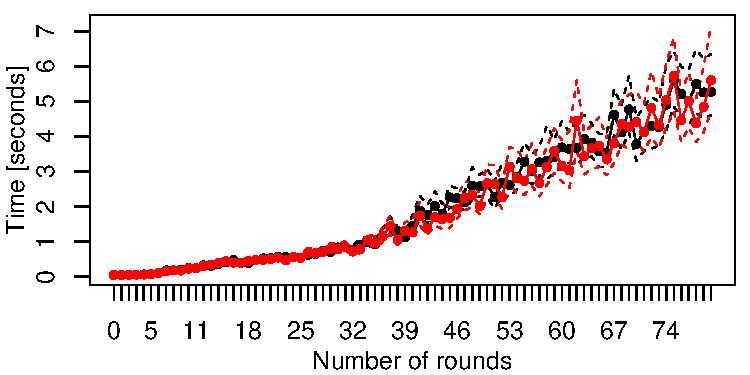
\includegraphics[width=\columnwidth]{figures/opt-sha1/sha1-32bit-8bitref-cmp-espresso-sq-lin.pdf}

The black points are without the choice function optimization, the red ones with.
We can see that while the optimization might reduce number of clauses (and therefore the instance size) it has no effect on the solving time.
Statistical analysis using the \emph{Games-Howell} procedure \cite{games1976pairwise} confirms this.
~\\

We also performed a very similar experiment on \emph{SHA-3-512}, optimizing two different expressions.
However the results were the same -- the optimizations did lead to smaller instances but not faster solving.
~\\

From this we conclude that using our library in the most straightforward way with minimal changes to existing implementations is sufficient for good performance.


%\mysection{Library}
%TODO link+qr
%TODO selected references


%%% zoznam literatury
\bibliographystyle{alpha}
\bibliography{research}

\end{multicols*}
\end{document}

